\section{Feasibility: How Much of an Erasure Fits in a Collision?}
\label{sec:feasibility}
We compute the deployed-collision box of Proposition~\ref{prop:box} for every edited
tensor and solve~\eqref{eq:capacity} with fit prompts disjoint from the evaluation
prompts (Appendix~\ref{app:recipe}). The W8A8 box uses the deployer's 128-caption
calibration statistics. Table~\ref{tab:capacity} reports five quantities per recipe:
\begin{itemize}
\item the fraction of edited coordinates whose edit fits inside the box, and the
median ratio of edit magnitude to the available slack in the edit's direction;
\item the passive explained fraction $f$ of the honest edit after quantization,
$\langle(\mathcal{Q}(W_E)-\mathcal{Q}(W_0))E,\Delta E\rangle/\|\Delta E\|^2$;
\item $f$ for coordinate-wise projection ($G=I$) and for the optimal reconstruction, on
held-out concept prompts;
\item the certified lower bound on the fit residual $\rho^*$; and
\item the minimum code agreement after the deployer recalibrates on the shipped
FP32 attack checkpoint.
\end{itemize}

\begin{table*}[t]
\centering
\caption{Collision feasibility for UCE erasure. \emph{Fits}: median fraction of edited
coordinates inside the collision box; \emph{Edit/slack}: median ratio of edit magnitude
to directional slack. $f$ is the explained fraction of the edit's key/value displacement
on held-out concept prompts (1 = full erasure effect, 0 = original model).
$\rho^*\ge$: certified lower bound on the optimal residual over fit prompts.
\emph{Agree}: minimum code agreement after deployer recalibration.}
\label{tab:capacity}
\begin{tabular}{lrrrrrrr}
\toprule
Recipe & Fits & Edit/slack & $f$ passive & $f$ projection & $f$ optimal & $\rho^*\ge$ & Agree\\
\midrule
\tableinput{data/capacity_rows.tex}
\bottomrule
\end{tabular}
\end{table*}

\begin{figure}[t]
\centering
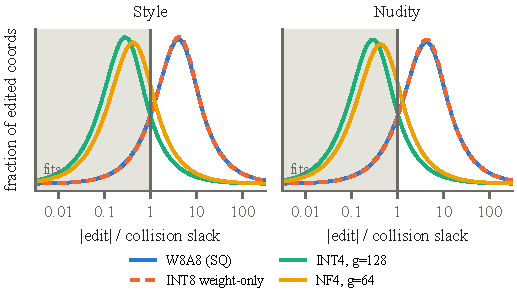
\includegraphics[width=\columnwidth]{figures/coord_slack.pdf}
\caption{Per-coordinate UCE edit magnitude relative to the collision slack in the
edit's direction, pooled over the 32 edited tensors. Coordinates left of 1 (shaded)
fit inside the deployed-collision box. At 8 bits the median edit is about four times
the slack; at 4 bits most edits fit.}
\label{fig:coords}
\end{figure}

\paragraph{8-bit grids leave little room}
Under SmoothQuant W8A8, only 16\% of edited coordinates fit in the box, and the
median edit is 3.9--4.0$\times$ the available slack (Figure~\ref{fig:coords}). The
optimal reconstruction reproduces 34\% (style) and 42\% (nudity) of the edit's
key/value displacement on held-out prompts, and the certificate is tight: no point of
$\mathcal{B}_{\pi_0}$ attains a fit residual below 0.696 (style) or 0.639 (nudity),
within $10^{-3}$ of what the solver achieves. Weight-only INT8 gives nearly identical numbers (34\% and 43\%). The barrier
is the resolution of the 8-bit grid, not SmoothQuant's activation-dependent
migration; calibration dependence neither helps nor hurts the attacker appreciably.

\paragraph{The earlier failure, explained}
Coordinate-wise projection, the repair step of our earlier construction, reproduces
only 11--12\% of the edit at 8 bits. Its measured FP16 scores (0.842 style, 0.574--0.583
nudity; Appendix~\ref{app:earlier}) are close to the original model's. The earlier
stealth failure is thus a property of the 8-bit collision box. More iterations could
not have fixed it.

\paragraph{4-bit grids are within reach}
Weight-only 4-bit bins are about $127/7\approx18$ times wider relative to their
group maximum. Under INT4 with groups of 128, 83--84\% of edited coordinates fit
(median edit/slack 0.27), and the optimal reconstruction reproduces essentially the whole
edit on held-out prompts ($f=1.00$ style, $0.99$ nudity; certified fit residuals
0.041 and 0.056). NF4 with groups of 64 is slightly tighter ($f=0.99$ and $0.98$).
Coordinate-wise projection is markedly weaker at 4 bits (0.67--0.79), so the
Gram-metric optimization matters exactly where an attack is feasible.

\paragraph{Passive quantization keeps the edit}
At every precision, the honest edit's output displacement survives
($f$ between 0.995 and 1.001), even though 15\% (8-bit) to 84\% (INT4) of edited
coordinates keep their original codes. The rank-limited closed-form edit is carried
by coordinates with large, aligned changes, which do move to new codes. Coordinate
reversion, the mechanism behind quantization-induced recovery of unlearned LLM
knowledge~\cite{zhang2025}, does not imply output reversion here.

\paragraph{A second closed-form editor}
We also computed the analysis for TIME~\cite{time} with the same phrase pairs. At these
settings the regularizers are small relative to $\|c_i\|^2$, so both editors reduce to
near-exact redirection of the phrase embeddings. Their edits, and every quantity in
Table~\ref{tab:capacity}, agree to three decimals. We therefore do not count TIME as
independent evidence.
